\documentclass[11pt,twoside,a4paper]{article}
\usepackage[utf8]{inputenc}
\usepackage{titlesec}
\usepackage[hidelinks]{hyperref}
\usepackage{graphicx}
\usepackage{pdfpages}
\usepackage[official]{eurosym}

\newcommand{\sectionbreak}{\clearpage}
\renewcommand\contentsname{Inhaltsverzeichnis}
\renewcommand\listfigurename{Abbildungsverzeichnis}
\renewcommand\listtablename{Tabellenverzeichnis}
\renewcommand\figurename{Abbildung}
\renewcommand\tablename{Tabelle}

\begin{document}
\pagenumbering{roman}
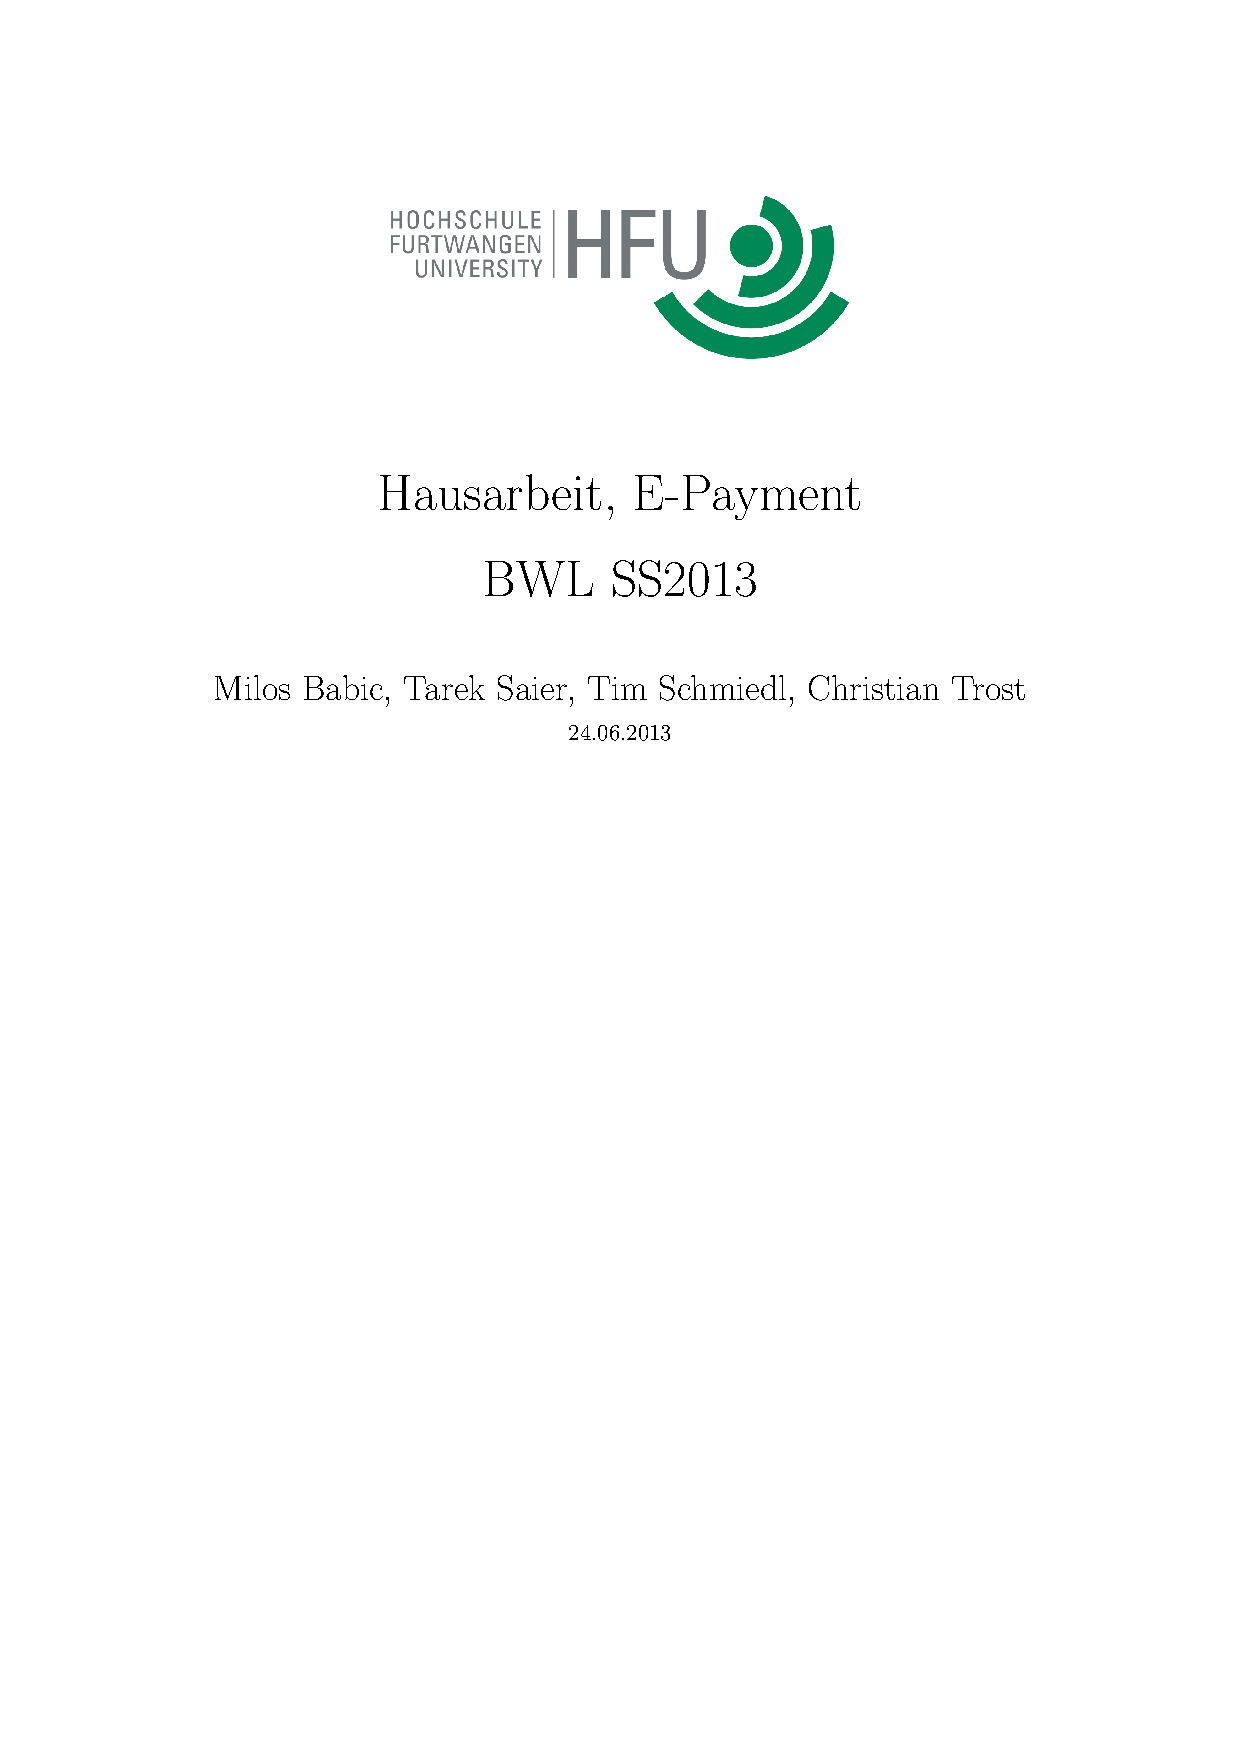
\includepdf{pdf/titlepage.pdf}

\clearpage
\setcounter{page}{1}

\begingroup
\let\clearpage\relax
\addcontentsline{toc}{section}{Inhaltsverzeichnis}
\tableofcontents
\phantomsection
\addcontentsline{toc}{section}{Abbildungsverzeichnis}
\listoffigures
\phantomsection
\addcontentsline{toc}{section}{Tabellenverzeichnis}
\listoftables
\endgroup

\clearpage
\pagenumbering{arabic}
\section{Einleitung}
\subsection{subsection}
\subsubsection{subsubection}
\paragraph{paragraph}
Hier dann einfach Text\\
manueller Zeilenumbruch.
\begin{enumerate}
	\item enumerate
	\item Aufzählung
	\item \textbf{Manchmal}\\
	Auch mit "Überschrift" nett
\end{enumerate}
\begin{itemize}
	\item itemize
	\item Stichpunkte
\end{itemize}
\textbf{fett}, \emph{kuziv}, \texttt{monospace}, Fußnote\footnote{foo bar}, Link-Fußnote\footnote{\url{http://www.google.com/}}
\begin{figure}[htb]
\centering
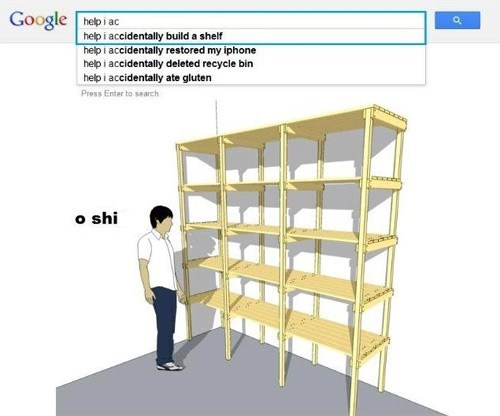
\includegraphics[width=\textwidth]{img/foo.png}
\caption{Abbildung mit Caption}
\label{fig:foo_00}
\end{figure}
Verweis auf Abbildung \ref{fig:foo_00} auf Seite \pageref{fig:foo_00}.

\clearpage
\section{Definitionen}

In diesem Kapitel werden Begrifflichkeiten erklärt, die für die Recherchen der Online-Bezahldienste und deren marktwirtschaftlichen Analyse von Nutzen sein können. 

\subsection[E-Payment]{E-Payment\footnote{\url{ https://de.wikipedia.org/wiki/Elektronisches_Geld}}}

E-Payment steht für Electronic Payment und bezeichnet eine neue Erscheinungsform des Geldes. Die offizielle Definition in Europa lautet:
\begin{quote}
``E-Geld-Richtlinie, 2000/46 EG: ein monetärer Wert in Form einer Forderung gegen die ausgebende Stelle, der
\begin{itemize}
	\item auf einem Datenträger gespeichert ist,
	\item gegen Entgegennahme eines Geldbetrags ausgegeben wird, dessen Wert nicht geringer ist als der ausgegebene monetäre Wert,
	\item von anderen Unternehmen als der ausgebenden Stell als Zahlungsmittel akzeptiert wird.''
\end{itemize}
\end{quote}



\subsubsection{Erscheinungsformen von E-Geld}

\paragraph{Karten gestütztes E-Geld}oder auch Kartengeld genannt, beinhaltet das E-Geld auf einer Karte mit Chip oder Magnetstreifen. In Deutschland ist die Geldkarte\footnote{\url{  https://de.wikipedia.org/wiki/Geldkarte}} das bekannteste Beispiel. Auf der Chipkarte ist das Guthaben gespeichert, welches dann zur Bezahlung verwendet werden kann.

\paragraph{Software basiertes E-Geld}bzw. Netzgeld wird über ein Rechnernetz transferiert. Das E-Geld befindet sich entweder auf einer Festplatte oder einem Online-Konto, welches dann zwischen zwei Rechnern transferiert wird. Der Online-Bezahl-Dienstleister PayPal transferiert Netzgeld mittels Online-Konten der jeweiligen registrierten Benutzer.
%https://de.wikipedia.org/wiki/Elektronisches_Geld

\subsubsection{Elektronische Zahlungssysteme}
%https://de.wikipedia.org/wiki/Elektronisches_Geld
Kategorisieren lassen sich elektronische Zahlungssysteme nach folgenden Betrachtungsweisen:
\paragraph{Zeitpunkt}
\begin{itemize}
     \item Prepaid: Zahlung wird vor dem Kauf ausgeführt
     \item Pay Now: Zahlung bzw. Abbuchung vom Kundenkonto wird zeitgleich mit dem Kauf ausgeführt
     \item Pay Later: Kundenkonto wird erst nach der Transaktion belastet.
\end{itemize}

\paragraph{Höhe des Betrags}
\begin{itemize}
     \item Macropayment: Zahlungen ab ca. \EUR{5}
     \item Micropayment: Zahlungen von ca. \EUR{0.05} bis ca. \EUR{5}
     \item Milipayment bzw. Minipayment: Zahlungen bis ca. \EUR{0.05}
\end{itemize}

\paragraph{Eingesetzter Hard- und Software:} Kategorisieren nach den eingesetzten Hard-/Software-Komponenten

\paragraph{Mischkategorisierung}
Die Kategorisierung reicht heutzutage nicht mehr aus, um die E-Payment-Systeme überschaubar abzugrenzen. Sie vermischen sich in den Kategorien zu sehr. Um die Dienstleister weitestgehend über\-sichtlich abzugrenzen, entwickelte Knud Bähle die folgende Mischkategorisierung:
\\
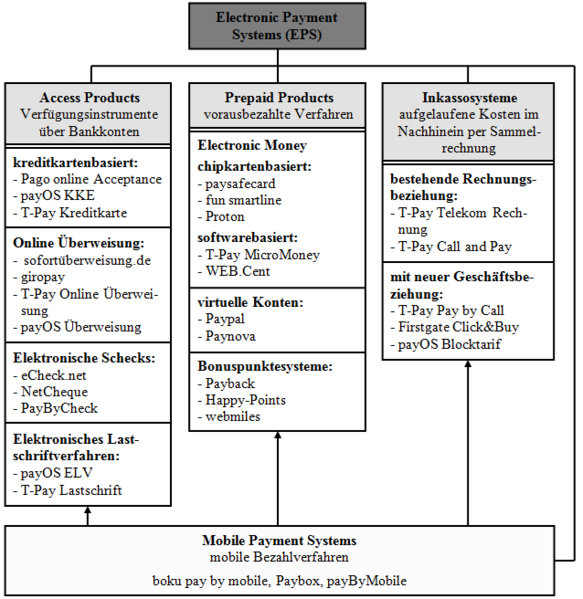
\includegraphics[]{img/Mischform.png}

\paragraph{Access Products} führen ihre Zahlungen über reale Bankkonten. Der Kunde gibt die benötigten Informationen seines Bankkontos an den Dienstleister. Online-Zahlungen mittels Kreditkarten, elektronischer Schecks oder Lastschriftverfahren führen auf das beschriebene Bankkonto zurück.

\paragraph{Prepaid Products} bieten E-Geld an, welches gegen reales Geld getauscht wird. Der Kunde hat somit sein reales Guthaben für Online-Zahlungen als E-Geld zur Verfügung stehen. Das Guthaben bzw. das E-Geld ist dann in Form von Chipkarten, Netzgeld oder auf einem virtuellem Konto gespeichert.

\paragraph{Inkassosysteme} schicken aufgelaufene Kosten nach Transaktionen per Sa\-mmelrechnung. 

\paragraph{Mobile Payment Systems} sind Bezahlsysteme, bei welchem Beträge über Mobilfunktelefone beglichen werden können. Klingeltöne oder Bilder, die man über eine SMS an den jeweiligen Anbieter als Bestellung gesendet hat, wird von der PrePaid-Karte abgebucht oder bei Mobilnetzverträgen auf die Rechnung hinzu addiert.\footnote{\url{ https://de.wikipedia.org/wiki/Handypayment}}



\subsection[Die Vision eines Unternehmens]{Die Vision eine Unternehmens\footnote{\url{ http://www.sunternehmensentwicklung.de/vision-unternehmen/uncategorised/vision-unternehmen.html}}}

Eine Unternehmensvision beschreibt ein in der Zukunft liegenden erstrebenswerten Zustand bzw. die zukünftige Entwicklung des Unternehmens. Sie erzielt je nach Betrachtungsweise verschiedene Effekte: Die Mitarbeiter des Unternehmens identifizieren sich mit der Vision und dem Unternehmen selbst. Die Langfristigen Ziele des Unternehmens sollen für jeden Mitarbeiter allgegenwärtig sein und den Sinn der eigenen Tätigkeit bewusst machen. Es fördert somit die Motivation und den Spaß an der Arbeit. Bei Kunden weckt eine Vision das Interesse an ein Unternehmen und verleiht einen souveränen Eindruck: Die Vision vermittelt Vertrauen.
 

\subsection[Geschäftsmodell]{Geschäftsmodell\footnote{\url{ http://de.wikipedia.org/wiki/Geschaeftsmodell}}}

Ein Geschäftsmodell ist eine modellhafte Beschreibung über die logische Funktionsweise eines Unternehmens. Es beantwortet folgende Fragen hinsichtlich der drei Hauptkomponenten:
\begin{itemize}
	\item Nutzerversprechen: Welchen Nutzen und Wert stiftet das Unternehmen für Kunden und seinen strategischen Partnern?
	\item Architektur der Wertschöpfung: Wie erbringt das Unternehmen diesen Nutzen?
	\item Ertragsmodell: Wodurch erwirtschaftet das Unternehmen seine Gewinne?
\end{itemize}

Geschäftsmodelle helfen bei der Analyse des Unternehmens. Es kann Schlüsselfaktoren herausfinden und die Gründe für einen Erfolg oder Misserfolg eines Unternehmens erklären.


\subsection[Kernkompetenz]{Kernkompetenz \footnote{\url{ http://de.wikipedia.org/wiki/Kernkompetenz}}}

Unter einer Kernkompetenz versteht man eine Fähigkeit eines Unternehmens, die im Vergleich zur Konkurrenz besser ausgeführt wird und dadurch einen Wettbewerbsvorteil erlangt. Jedes Unternehmen besitzt eine Kernkompetenz, auf welches es sich stützt und versucht, diese weiter auszubauen. Je nach Unternehmenslage kann ein Unternehmen seine Kernkompetenzen aus- oder abbauen oder auch das Repertoire an Kernkompetenzen erweitern oder verringern.
\subsubsection{Kernkompetenzen identifizieren}
Kernkompetenzen können identifiziert werden. Um diese zu finden, können folgende Eigenschaften einer angeblichen Kernkompetenz untersucht werden:
\begin{itemize}
\item Differenzierung: besitzt die Kernkompetenz das Potential, einen nachhaltigen Vorteil gegenüber der Konkurrenz zu führen?
\item Diversifikation: bietet die Kernkompetenz Zugang zu neuen Märkten?
\item Kundennutzen: hat der Kunde einen nachhaltigen Mehrwert durch diese Kernkompetenz?
\item Imitationsschutz: kann die Kernkompetenz von der Konkurrenz leicht imitiert werden?
\end{itemize}




\subsection[Kritischer Erfolgsfaktor]{Kritischer Erfolgsfaktor \footnote{\url{ http://de.wikipedia.org/wiki/Kritischer_Erfolgsfaktor}}}

Kritische Erfolgsfaktoren sind Eigenschaften, die bei einem Unternehmen bei guten Werten das Erreichen ihrer Ziele ermöglicht. Sie entscheiden über den Erfolg eines Unternehmens. In einem IT-Projekt entscheiden gutes Projekt- und Risikomanagement, sowie auch das Entwicklungsteam zum Erfolg des Projektes selbst und somit auch der des Unternehmens.



\subsection[Strategie]{Strategie\footnote{\url{ http://de.wikipedia.org/wiki/Strategie_(Wirtschaft)}}}
Eine Strategie im Wirtschafts-Kontext ist eine geplante Verhaltensweise eines Unternehmens um ihre Ziele zu erreichen. Sie legt fest, in welchen Aktivitätsfelder das Unternehmen tätig sein soll. Strategien richten sich auf das gesamte Unternehmen und spiegeln die zentrale Einstellungen, Wünsche und Wertvorstellungen der bestimmenden Entscheidungsträger des Unternehmens wider. Es bezieht sich auf das Umfeld und der Konkurrenz: Soll eine Fusion mit der Konkurrenz erfolgen? Gibt es eine Möglichkeit, sich von der Konkurrenz abzugrenzen? Kann man Kernkompetenzen der Konkurrenz imitieren? 



\subsection[Indikatoren]{Indikatoren\footnote{\url{ http://de.wikipedia.org/wiki/Indikator_(Wirtschaft)}}}

Indikatoren sind im Allgemeinem Messgrößen, die zur Steuerung und Orientierung einer Organisation helfen. Sie beschreiben einen Zustand oder quantifizierbaren Wert. In der Wirtschaft unterscheidet man zwischen volkswirtschaftlichen und betriebswirtschaftlichen Indikatoren bzw. Kennzahlen.

\subsubsection{Volkswirtschaftlicher Indikator [9]}

Volkswirtschaftliche Indikatoren werden auch Konjunkturindikatoren oder makroökonomische Kennzahlen genannt. Ihre Werte beschreiben die wirtschaftliche Situation im Allgemeinen von Volkswirtschaften und können als Basis für die Erstellung von Wirtschafts-Prognosen eingesetzt werden. 
\\
Konjunkturindikatoren eignen sich zur Bewertung von Aktien, weil sie Rück\-schlüsse aus der gesamtwirtschaftlicher Entwicklung ziehen, die wiederum die wirtschaftliche Situation einzelner Industriesektoren abbilden. Konjunkturindikatoren lassen sich in drei Kategorien aufteilen:

\paragraph{Mengenindikatoren} informieren über die Mengenentwicklung eines Bezugsobjektes, wie zum Beispiel Arbeitslosenzahl, Auftragseingänge oder Industrieproduktion.
\paragraph{Preis- bzw. Kostenindikatoren} beschreiben das Preisniveau bzw. die Entwicklung eines Bezugsobjektes. Dazu gehören Aktienkurse, Immobilienpreise, Lebensmittelpreise und Rohstoffpreise.
\paragraph{Früh-, Präsenz- und Spätindikatoren} beschreiben den zeitlichen Vor- bzw. Nachlauf eines Sachverhaltes. 

Frühindikatoren weisen auf zukünftige Entwicklung der Wirtschaftslage. Dazu gehören der Aktienindex, Rohstoffindex, Gewinnerwartungen und Einzelhandelsumsätze. 

Präsenzindikatoren geben Auskunft über die aktuelle Wirtschaftsentwicklung: Bruttoinlandsprodukt, Industrieproduktion, Kurzarbeit und Lagerbe\-stände.

Spätindikatoren beschreiben die Wirtschaftsentwicklung in der Vergangenheit: Arbeitslosenquote, Inflationsrate, Insolvenzen, Lohnentwicklung, Steu\-ereinnahmen des Staates.

\paragraph{Wachstumsrate} bzw. Inflationsrate stellen absolute Größen dar, wie den Stand eines Aktienindex, Logistikindex oder Rohstoffindex.
   

\subsubsection[Betriebswirtschaftlicher Indikator]{Betriebswirtschaftlicher Indikator \footnote{\url{http://de.wikipedia.org/wiki/Betriebswirtschaftliche_Kennzahl}}}
Betriebswirtschaftliche Indikatoren dienen zur Beurteilung von Unternehmen innerhalb der Betriebswirtschaft. Folgende Funktionen können diese Kennzahlen besitzen:

\paragraph{Entscheidungsfunktion:} Entscheidungsträger können anhand von Kennzahlen betriebswirtschaftliche Entscheidungen treffen. Kennzahlen können auf Probleme oder Chancen hinweisen.
\paragraph{Kontrollfunktion:} Kennzahlen können der Kontrolle des Gesamterfolges des Unternehmens dienen.
\paragraph{Koordinationsfunktion:} helfen bei der Durchsetzung von Entscheidungen über die Koordination verschiedener unternehmerischer Bereiche und bei der Verhaltenssteuerung von Mitarbeitern.
\paragraph{Verhaltenssteuerungsfunktion:} zum Motivieren der Mitarbeiter zu einer für das Unternehmen positiven Verhaltensweise.

\newpage

\paragraph{Arten von Kennzahlen}
\subparagraph{Absolute Kennzahlen} drücken einen betriebswirtschaftlichen Einzelwert aus. Sie stehen in keine Relation zu anderen Kennzahlen. Zu diesen Arten von Kennzahlen gehören beispielsweise Summenwerte, Differenzwerte und Mittelwerte.
\subparagraph{Relative Kennzahlen} entstehen durch eine Relation zweier betriebswirtschaftlicher Werte zu einer Kennzahl, die einen erhöhte oder spezifische Aussagekraft besitzt.

\subsubsection{Gliederung von betriebswirtschaftlichen Kennzahlen}
Kennzahlen lassen sich nach dem zugrunde liegenden Sachverhalt, der durch sie ausgedrückt werden soll, gliedern.

\paragraph{Erfolgskennzahlen} dienen der Ermittlung des Unternehmenserfolgs und orientieren sich am Gewinn oder am Unternehmenswert. Zu Erfolgskennzahlen gehören Umsatz, Cashflow, Produktergebnis,, Gesamtbetriebsertrag, Rohertrag und Gewinne vor Steuern.

\paragraph{Liquiditätskennzahlen} geben Informationen über den Zustand der Zahlungsmöglichkeit eines Unternehmens an, um seine fälligen Verbindlichkeiten begleichen zu können. Kennzahlen wie Cash Ratio, Anlagendeckung und Einzugsliquidität gehören zu Liquiditätszahlen.\footnote{\url{http://www.wirtschaftslexikon24.com/d/liquiditaetskennzahlen/liquiditaetskennzahlen.htm}}


\paragraph{Rentabilitätskennzahlen} beschreiben das Verhältnis einer Erfolgsgröße zum eingesetztem Kapital: Gesamtkapitalrentabilität, Eigenkapitalrentabilität und Umsatzrendite. \footnote{\url{http://de.wikipedia.org/wiki/Rentabilitaet}}

\paragraph{Bilanzkennzahlen} oder Kennzahlen zur Kapitalstruktur geben Auskunft über die Bilanz eines Unternehmens, zum Beispiel Eigenkapitalquote, Fremdkapitalquote, Verschuldungsgrad und Anlagenintensität.

\paragraph{Kennzahlen zur Umschlagshäufigkeit} wie Kapital- und Lagerumschlags\-häuigkeit, beschreiben, wie oft ein Wert sich in einem bestimmten Zeitraum wiederholt.
    
 



\subsection[Marktanalyse]{Marktanalyse \footnote{\url{http://de.wikipedia.org/wiki/Marktanalyse}}}

Die Marktanalyse dient der Darstellung der aktuellen Marktsituation. Es werden Daten erhoben, die gerade aktuell sind und so für Entscheidungen herangezogen werden können. Die Daten stammen aus internen Marktdaten, wie Verkaufszahlen oder Produktionskosten und externen Marktdaten wie makroökonomische Trends. Aus der Analyse können Marketingpläne erstellt werden, aus denen strategische Ziele und Maßnahme abgeleitet werden können.
\\
Zu Marktanalysen gehören folgende Recherchen dazu:
\begin{itemize}
	\item Marktpotential bei innovativen Produkten oder Dienstleistungen
	\item Marktvolumen und Marktentwicklung
	\item Marktstruktur nach Teilmärkten in Regionen/Ländern, Produktgruppen oder Kundentypen
	\item Konkurrenzanalyse
	\item Produktlebenszyklusanalyse 
\end{itemize}



\subsection[Konkurrenzanalyse]{Konkurrenzanalyse \footnote{\url{http://de.wikipedia.org/wiki/Konkurrenzanalyse}}}
In der Konkurrenzanalyse werden Informationen über Konkurrenzunternehmen systematisch und legal gesammelt und ausgewertet. Dabei werden ihre Produkte, Marktentwicklungen, neue Patente und Technologien beobachtet und analysiert. Es ist ein wichtiger Bestandteil der Marktanalyse und ermöglicht Unternehmen eine frühzeitige Anpassung ihrer Strategie um somit Wettbewerbsvorteile zu erreichen.
%\section{Technologien und Zahlprozesse}

\subsection{Einzahlung}
Für alle Online-Bezahldienste muss natürlich eine Geldquelle hinterlegt sein. Das Bezahlen kann über eine der drei Möglichkeiten geschehen: "Pre-Paid", "Pay-now", "Pay-later".\\
Guthabenbasiertes Bezahlen(Pre-Paid) findet man z.B. bei Paypal. Hier kann per Überweisung auf ein virtuelles Konto eingezahlt werden. Nach Geldeingang kann über das Geld in diesem Konto verfügt und damit Bezahlungen getätigt werden.
Ebenfalls sehr verbreitet (vor allem in den USA) ist das Hinterlegen von Kreditkarten oder Debitkarten. Eine weitere Möglichkeit ist das Hinterlegen der Kontodaten und Bezahlen über Lastschrift.\footnote{\url{http://en.wikipedia.org/wiki/Online_wallet}}

\subsection{Bezahlmöglichkeiten}
\subsubsection{Web}
\textbf{Virtulles Konto}\\
Ein virtuelles oder Online-Konto fungiert als Zwischenglied zwischen Kundenkonto und Verkäufer. Oftmals kann der Kunde von seinem Konto aus im Voraus Überweisungen tätigen (Pre-Paid), welche dann auf dem virtuellen Konto gutgeschrieben sind. Oftmals werden auch über Lastschrift oder Hinterlegen von Kreditkarteninformationen zusätzliche Zahlungsmöglichkeiten geschaffen.\\
Überweisungen zwischen verschieden (virtuellen) Konten ist oftmals auch möglich.\\
Als Beispiel hierfür ist u.A. Paypal zu nennen.\footnote{\url{http://paypal.com}}

\textbf{Checkout via Provider}\\
Der vermutlich "gewöhnlichste" Bezahlvorgang. Hierbei werden beim jeweiligen Provider Konto-/Kreditkartendaten hinterlegt. Diese sind dann dort gespeichert und werden für Abbuchungen verwendet.
Der jeweilige Provider übernimmt dabei den gesamten Bezahlvorgang. Ein Bezahlvorgang sieht meist folgendermaßen aus: der Kunde legt in einem Webshop einen Artikel in den Warenkorb und wählt die Bezahlung über den jeweiligen Provider aus. Somit ist der Vorgang für ihn abgeschlossen. Der Verkäufer erhält schließlich das Geld vom Provider, abzüglich der Transaktionskosten.\\
Beispiele hierfür ist u.A. Amazon Payments.\footnote{\url{https://payments.amazon.com/sdui/sdui/business/cba}}\\

\textbf{Kreditkarte}\\
Ebenfalls möglich ist auch eine direkte Bezahlmöglichkeit über Kreditkarte. Hierbei muss der Kunde seine Kreditkartendaten direkt an den Verkäufer übermitteln. Dabei ist neben dem Kreditkarteninstitut kein weiterer Partner beteiligt. Jedoch hier für den Kunden problematisch ist, dass er seine Kartendaten einer weiteren Partei zur Verfügung stellen muss. Für den Verkäufer gibt es eventuell die Gefahr von nicht gedeckten Karten.\\

\textbf{Email}\\
Neu von Google Wallet eingeführt ist das Versenden von Geld via Email. Dabei muss der Absender einen Wallet-Account haben und kann damit mit sein GMail-Konto Geld an beliebgige Personen versenden. Der Empfänger bekommt das Geld ebenfalls auf ein Wallet-Account übertragen. Hat er diesen nicht, so muss er sich erst registrieren um über das Geld verfügen zu können.\footnote{\url{http://www.google.com/wallet/send-money/}}\\

\subsubsection{Mobile}
\textbf{Mobile Web Payments\footnote{\url{http://en.wikipedia.org/wiki/Mobile_phone_micropayment\#Mobile_web_payments_.28WAP.29}}}\\
Eine einfache Möglichkeit mobil bezahlen zu können, ist die einfache Adaption von ePayment-Webanwendung für mobile Devices. Über WLAN oder mobiles Internet kann die Verbindung zu einem Webserver hergestellt werden. Die Vorgänge gleichen dabei den Abläufen einer Desktop-Anwendung.\footnote{\url{http://link.springer.com/chapter/10.1007/978-3-642-29802-8_9/fulltext.html\#Sec15}}\\

\textbf{Premium SMS\footnote{\url{http://en.wikipedia.org/wiki/Mobile_phone_micropayment\#SMS.2FUSSD-based_transactional_payments}}}\\
Eines der ältesten mobilen Bezahlmöglichkeit ist die sogenannten Premium SMS. Über das Senden von SMS an kostenpflichtige Nummern kann Geld transferiert werden. Dabei bezahlt der Kunde über seine Telefonrechnung. Hierbei spielt der Netzprovider die Vermittlungsrolle zwischen Kunde und Verkäufer.\\
Besonders in Europa und Asien war und ist diese Variante des mobilen Bezahlens weit verbreitet, wird jedoch nach und nach durch neuere Möglichkeiten ersetzt. Vor allem die hohen Abgaben an den Mobilfunkprovider von bis zu 40-50\% sind ein Grund hierfür.\\
Verwendet wird es vor allem für sehr kleine Beiträge (Micropayment) wie z.B. für Klingeltöne, Logos oder TV-Votings. Es gab jedoch auch einige ausgefallenere Beispiele, wie etwa das Programm "Dial-a-coke" von der Coca Cola Company: Ein Kunde kauft an einem Getränkeautomaten ein Erfrischungsgetränk und bezahlt es mit seinem mobilen Telefon. Dazu ruft er eine auf dem Automaten stehende Nummer an und wählt anschließend an seinem mobilen Telefon ein Produkt aus. Das ausgewählte Produkt wird vom Automaten ausgegeben, die Bezahlung erfolgt über die Telefonrechnung.\footnote{\url{http://link.springer.com/chapter/10.1007/978-3-642-29802-8_9/fulltext.html\#Sec15}}\\
 
\textbf{Direct mobile billing}\\
Verwandt mit dem Premium SMS, verwendet auch "Direct mobile billing" den Mobilfunkanbieter als Zwischenhändler.\\
Typischerweise gibt hier der Kunde dem Verkäufer seine Handynummer an und erhält dann nach kurzer Zeit eine SMS mit einem bestimmten Code. Diesen kann er schließlich auf einer Webseite oder einer App eingeben um so den Kaufvorgang abzuschließen. Belastet wird hierbei wieder die Telefonrechnung.
Trotz hohen Abgaben von 10-20\% an den Netzanbieter steigt der Umsatz dieser Bezahlmethode aufgrund der Einfachheit in den letzten Jahren kontinuierlich weiter. Inzwischen wird diese Methode von großen Unternehmen wie Facebook oder Zynga eingesetzt.\footnote{\url{http://usatoday30.usatoday.com/tech/news/story/2012-04-04/mobile-billing-boku-zong/54003414/1}}\\


\textbf{NFC}\\
Near Field Communication\footnote{\url{https://de.wikipedia.org/wiki/Near_Field_Communication}}, kurz NFC ist eine Technik zum kontaktlosen Austausch von Daten über sehr kurze Strecken, typischerweise von wenigen Zentimetern. Diese kurze Reichweite ist erwünscht um den Kunden mehr Sicherheit zu bieten. So muss das Smartphone mit NFC-Chip oftmals direkt auf das Lesegerät gelegt bzw. daran gehalten werden. \\
Da die Technologie noch relativ neu ist, gibt es vorerst nur wenige Geräte mit NFC-Unterstützung. Doch besonders mit dem mobilen Betriebsystem Android scheint die Technologie langsam Fuß zu fassen. So wurde mit dem "Android Secure Element" und seiner API\footnote{\url{https://code.google.com/p/seek-for-android/}} ein eigenes Modul mitsamt Chipsatz und externen Speicher geschaffen um das sichere Speichern von sensiblen Daten, wie sie beim NFC anfallen, zu ermöglichen.\footnote{\url{http://link.springer.com/content/pdf/10.1007\%2F978-3-642-30436-1_1.pdf}}\\
Anbieter, welche auf auf diese Technologie setzten, sind neben schon erwähnten Google Wallet auch das von Deutscher Bahn und Vodafone geschaffene Programm Touch\&Travel, oder die Sparkasse girogo, welche damit Zahlungen bis 20€ anbietet.
Seit 2011 ist auch der deutsche Personalausweis NFC-kompatibel.\footnote{\url{https://de.wikipedia.org/wiki/Near_Field_Communication\#Echteinsatz}}\\
Gefährlich - natürlich neben dem Verlust des NFC-Gerätes - kann das beiläufige Auslesen von Daten sein. Dies und der Schutz der Privatsphäre kann nur dann sichergestellt werden, wenn die Funktionen im Normalfall komplett abgeschaltet sind.\\

\textbf{QR-Code\footnote{\url{http://en.wikipedia.org/wiki/Mobile_phone_micropayment\#QR_Code_Payments}}}\\
QR-Codes erfreuen sich seit einiger Zeit großer Beliebtheit zur Übertragen von kurzen Informationen auf ein mobiles Gerät. Die weite Verbreitung und Einfachheit des Scann-Vorgangs findet auch in mobilen Bezahlsystemen ihren Einsatz. \\
Ein beispielhafter Vorgang könnte so ablaufen: der Kunde erhält an der Kasse einen QR-Code mit der Höhe des Betrages auf sein mobiles Gerät. Nun könnte er entweder auf eine Webseite geleitet werden um den Betrag zu bezahlen oder direkt mit einer App des Verkäufers zum Bezahlen aufgefordert werden.\\
Damit stellt es keine eigenständige Bezahlform dar, doch durch die Einfachheit des Scann-Vorgangs könnte sich das Verfahren noch weiter verbreiten. 
\clearpage
\section{Wertschöpfungskette}
foo bar

\clearpage
\section{Provider}


\clearpage
\section{Fazit}
Der E-Payment-Markt ist seit einigen Jahren ein sehr umsatzstarker Wirtschaftsbereich und gewinnt mit dem mobilen Payment einen weiteren, rasant wachsenden, Zweig hinzu. Es existieren heute eine Vielzahl von Möglichkeiten, seine Waren im Internet zu bezahlen. Diverse Provider bieten unterschiedliche Dienste und Technologien an um die Bedürfnisse verschiedener Kundengruppen zu befriedigen.\\
Besonders interessant sind die derzeitigen Entwicklungen im relativ jungen Markt des mobilen Payments. Fast jeder Bundesbürger besitzt heute ein Handy, wobei es sich dabei zu einem großen Teil um Smartphones mit mobilem Internet handelt. Durch diese hohe Marktdurchdringung ist das Potenzial in diesem Segment gewaltig. Dessen sind sich die Wettbewerber bewusst und bieten daher viele verschiedene Möglichkeiten der Bezahlung an bzw. entwickeln an Weiteren. Durch den rasanten technologischen Fortschritt der letzten Jahre in diesem Segment befinden wir uns hier noch in einer frühen Phase und können mit Spannung verfolgen wie es sich in den nächsten Jahren weiterentwickelt.\\
Dabei wird es von entscheidender Rolle sein, welche Aspekte dem Kunden am wichtigsten sind. So ist in einer Zeit, in welcher man fast täglich von Sicherheitslücken, Hackerangriffen und gestohlenen Informationen hört, die Sicherheit der Kundendaten eines der wichtigsten Anliegen des Kunden und daher bei den meisten Provider (zumindest vordergründig) großgeschrieben.


\end{document}
